\documentclass[letterpaper, 12pt]{article}
\usepackage[margin=0.45in]{geometry}
% \usepackage[moderate]{savetrees}
\usepackage{multicol}
\usepackage{paracol}
\usepackage{graphicx}
\graphicspath{{Figures/}{./}}
\usepackage{apacite}
\usepackage{amsmath}
\usepackage{derivative}
\usepackage{amssymb}
\usepackage{amsthm}
\usepackage{indentfirst}
\usepackage{siunitx}
\usepackage[justification=centering]{caption}
\usepackage{float}
\usepackage{url}
\usepackage{tabularray}

\pagenumbering{roman}

\title{PHYSICS SL
\\
Barton's Pendulum}
\author{}
\date{}

\begin{document}
\nocite{*}

\maketitle
\begin{center}
    Session: May 2024
    \\
    Page Count:
\end{center}
\newpage

\tableofcontents
\newpage

\pagenumbering{arabic}
\setcounter{page}{1}

\section{Research Question}

What is the relationship between the amplitude of
the forced pendulum /\unit{rad} and the
angular frequency of the driver pendulum /\unit{rad.s^{-1}} in a Barton's pendulum.

\section{Introduction}

Pendulums undergo a repeating cycle of energy transfer from
only potential energy to only kinetic energy back to
only potential energy. This process causes
a pendulum system to undergo simple harmonic motion,
therefore pendulums have properties such as
period and frequency of oscillation defined
that are dependent on the length of the pendulum.

What this also means is that any periodic
external force will or will not resonate with
the pendulum. This applies to various real-life
scenarios and problems, from something as little
as the frequency that a parent should push
their child on a swing to whether gusts
of wind are capable of driving an idle wrecking ball
to dangerous.

Intuitively, if an external periodic force
is resonant with the pendulum, then the extent
that the pendulum's amplitude will reach
will be at its maximum. However, one should question exactly
how this maximum amplitude grows as the frequency
of the external force approaches the resonant frequency
of the pendulum.

This could easily be investigated by suspending
a driving pendulum and a forced pendulum on
the same string. This allows for an easy way
to provide an external periodic force through
the driver pendulum, allowing for the frequency
of the external force to be manipulated through
changing the length of the driver pendulum and
removing the necessity of a motorized
instrument.

\section{Background information} \label{sec:bgInfo}

\subsection{Friction in a pendulum}

Because a pendulum is not sliding along a surface,
then friction cannot be defined by the formula
\(F_f = \mu F_N = \mu_d R\). However, a pendulum
behaves alike to a particle experiencing frictional force
that is proportional to its velocity \cite{FrictionalForceProportional2021}.
It can therefore be defined as

\begin{equation} \label{eq:frictionVelocity}
    F_f = -\gamma v
\end{equation}
\[
    \text{Where } \gamma = \text{the coefficient of friction of an object experiencing friction through drag } /\unit{kg.s^{-1}}
\]

Note that the negative sign is necessary, as the direction
of translational velocity of the pendulum
opposes the direction of frictional force.

\begin{figure}[H]
    \centering
    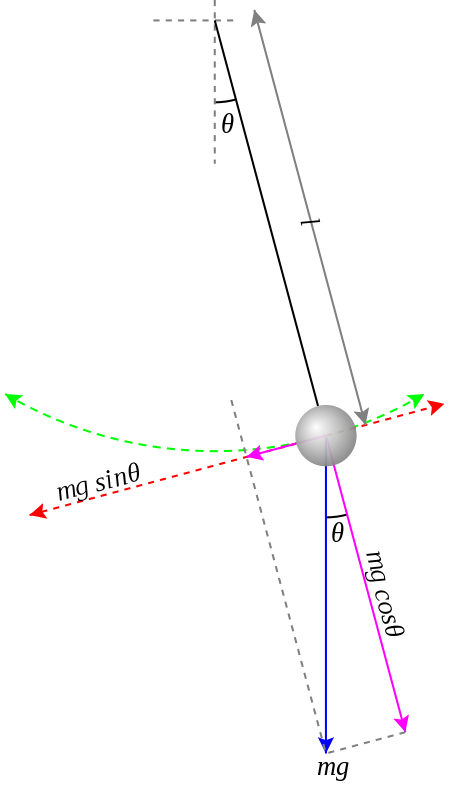
\includegraphics[width=0.3\textwidth]{labelledPendulum.png}
    \caption{Pendulum labelled with components of gravitational force \protect\cite{krishnavedalaEnglishDiagramDepicting2013}.}
    \label{fig:labelledPendulum}
\end{figure}

With reference to Figure \ref*{fig:labelledPendulum}, the
displacement along the green arc (\(s\)) can be defined
below using the definition of a radian.

\begin{equation} \label{eq:defineS}
    s = l\theta
\end{equation}
\[
    \text{Where } l = \text{the length of the forced pendulum } /\unit{m}
\]

Differentiating both sides of Equation \ref*{eq:defineS},
the following relationship is obtained.

\begin{equation}
    \dot s = v = l \dot \theta
\end{equation}

This means that Equation \ref*{eq:frictionVelocity} can be rewritten as
\begin{equation}
    F_f = -\gamma l \dot\theta
\end{equation}

\subsection{External periodic force on a pendulum}

The external periodic force on a pendulum can be modelled as follows

\begin{equation}
    F_e = A_e \cos (\Omega t)
\end{equation}

\begin{align*}
    \text{Where } F_e & = \text{the external periodic force acting on the pendulum } /\unit{N}
    \\
    A_e               & = \text{the amplitude of the external periodic force } /\unit{N}
    \\
    \Omega            & = \text{the angular frequency of the external periodic force } /\unit{rad.s^{-1}}
    \\
    t                 & = \text{duration of time passed after a reference moment in time } /\unit{s}
\end{align*}

\subsection{The Damped, Driven Pendulum}

In Figure \ref*{fig:labelledPendulum}, the component of
gravitational force parallel to the instantaneous velocity of
the pendulum is \(mg\sin\theta\). However, when letting
\(F_g\) equal to such component of gravitational force,
it must equal to the negative of \(mg\sin\theta\)
such that the directionality of \(F_g\) opposes
the directionality of the horizontal component
of \(s\).

\begin{equation}
    F_g = -mg\sin\theta
\end{equation}

% \begin{figure}[H]
%     \centering
%     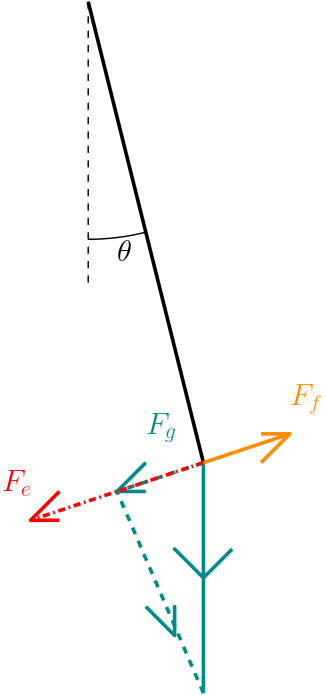
\includegraphics[width=0.2\textwidth]{forcesOnPendulum.png}
%     \caption{A pendulum with relevant forces labelled}
%     \label{fig:f_netPendulum}
% \end{figure}

With reference to Figure \ref*{fig:labelledPendulum}, Equation \ref*{eq:noApproximate}
can be derived as follows.

\begingroup
\allowdisplaybreaks
\begin{paracol}{2}
    \begin{align*}
         & F_{net}                                                   = ma
        \\
         & F_g + F_f + F_e                                           = ma
        \\
         & -mg\sin\theta - \gamma l\dot\theta + A_e \cos (\Omega t)  = m\ddot s \tag{A} \label{eq:simpleNewton}
        \\
        \\
         & m\ddot s                                                  = -mg \sin\theta
        \\
         & l\ddot \theta                                             = -g\sin\theta \tag{B} \label{eq:gsin}
        \\
         & \ddot\theta                                               = -\frac{g}{l}\sin\theta
        \\
         & \because \omega                                          = \sqrt{\frac{g}{l}}
        \\
         & \ddot\theta                                               = -\omega^2\sin\theta \tag{C} \label{eq:angAccel_Vel}
    \end{align*}
    \switchcolumn
    \begin{align*}
         & \text{Substituting \ref*{eq:gsin} into \ref*{eq:simpleNewton}}
        \\
         & ml\ddot\theta - \gamma l\dot\theta + A_e \cos (\Omega t)                = m\ddot s \tag{D} \label{gsinSubstituted}
        \\
         & \text{Substituting \ref*{eq:angAccel_Vel} into \ref*{gsinSubstituted}}
        \\
         & -ml\omega^2\sin\theta - \gamma l\dot\theta + A_e \cos (\Omega t)        = m\ddot s
        \\
         & \because \ddot s                                                        = l\ddot \theta
        \\
         & A_e\cos(\Omega t)                                                       = ml\ddot \theta + \gamma l\dot\theta + ml\omega^2\sin\theta
        \\
         & \text{Letting } C                                                       = \frac{A_e}{ml}
        \\
         & \lambda                                                                 = \frac{\gamma}{m}
    \end{align*}
\end{paracol}
\endgroup
\begin{equation} \label{eq:noApproximate}
    \ddot\theta + \lambda\dot\theta + \omega^2\sin\theta = C\cos(\Omega t)
\end{equation}

A formula to determine the amplitude of a damped, driven pendulum
can be then determined.

\begingroup
\allowdisplaybreaks
\begin{align*}
    \text{Using the small}                           & \text{ angle approximation of }    \sin\theta \approx \theta
    \\
    \ddot\theta + \lambda\dot\theta + \omega^2\theta & = C\cos(\Omega t)
    \\
    \ddot z + \lambda\dot z + \omega^2 z             & = Ce^{i\Omega t}
    \\
    \text{The ansatz for }                           & z \text{ is } Ae^{i\Omega t} ~\text{\cite{chasnov11DampedDriven2022}}
    \\
    \dot z = i\Omega Ae^{i\Omega t},                 & \quad \ddot z = -\Omega^2 Ae^{i\Omega t}
    \\
    -\Omega^2 A + i\lambda\Omega A + \omega^2 A      & = C
    \\
    A                                                & = \frac{C}{(\omega^2 - \Omega^2) + i\lambda\Omega} \times \frac{(\omega^2 - \Omega^2) - i\lambda\Omega}{(\omega^2 - \Omega^2) - i\lambda\Omega}
    \\
    A                                                & = \frac{C\left[ (\omega^2 - \Omega^2) - i\lambda\Omega \right]}{(\omega^2 - \Omega^2)^2 + \lambda^2\Omega^2}
    \\
    \text{Using the exponential}                     & \text{ form of complex numbers: } a + bi = re^{i\phi}
    \\
    (\omega^2 - \Omega^2) - i\lambda\Omega           & = e^{i\phi} \sqrt{(\omega^2 - \Omega^2)^2 + \lambda^2\Omega^2}
    \\
    A                                                & = \frac{Ce^{i\phi}}{\sqrt{(\omega^2 - \Omega^2)^2 + \lambda^2\Omega^2}}
    \\
    \theta (t)                                       & = \Re (Ae^{i\Omega t})
    \\
    \theta (t)                                       & = \Re (e^{i\Omega t} \frac{Ce^{i\phi}}{\sqrt{(\omega^2 - \Omega^2)^2 + \lambda^2\Omega^2}})
    \\
    \theta (t)                                       & = \Re (e^{i(\Omega t + \phi)}) \frac{C}{\sqrt{(\omega^2 - \Omega^2)^2 + \lambda^2\Omega^2}}
    \\
    \theta (t)                                       & = \left(\frac{C}{\sqrt{(\omega^2 - \Omega^2)^2 + \lambda^2\Omega^2}}\right) \cos(\Omega t + \phi)
\end{align*}
\endgroup

\begin{equation} \label{eq:unlinearized}
    A = \frac{C}{\sqrt{(\omega^2 - \Omega^2)^2 + \lambda^2\Omega^2}}
\end{equation}

Equation \ref*{eq:unlinearized} assumes that:
\begin{itemize}
    \item Due to the small angle approximation made, \(\theta\) does not exceed \(13.99^{\circ}\)
    \item The string connected to the weight is massless
\end{itemize}

All derivations and ideas within Section \ref*{sec:bgInfo} were with reference to \cite{chasnov11DampedDriven2022}.

\section{Hypothesis}

When the length of the driver pendulum equals to the length of the forced pendulum,
then the amplitude of the forced pendulum will be at its maximum as the two pendulums
are in resonance.

As the length of the driver pendulum approaches the length of the forced pendulum,
then the amplitude of the forced pendulum will approach that maximum from lower values.
\\

A more detailed hypothesis can be made by referring to and modifying Equation \ref*{eq:unlinearized}.
\begin{align*}
    A             & = \frac{C}{\sqrt{(\omega^2 - \Omega^2)^2 + \lambda^2\Omega^2}}
    \\
    A^2           & = \frac{C^2}{(\omega^2 - \Omega^2)^2 + \lambda^2\Omega^2}
    \\
    A^2           & = \frac{C^2}{\Omega^4 + (\lambda^2 - 2\omega^2)\Omega^2 + \omega^4}
    \\
    \frac{1}{A^2} & = \frac{\Omega^4 + (\lambda^2 - 2\omega^2)\Omega^2 + \omega^4}{C^2}
\end{align*}

\begin{equation} \label{eq:modified}
    \frac{1}{A^2} = \frac{1}{C^2}\Omega^4 + \frac{\lambda^2 - 2\omega^2}{C^2}\Omega^2 + \frac{\omega^4}{C^2}
\end{equation}

Unfortunately, Equation \ref*{eq:modified} cannot be manipulated further
to achieve a linearized form. However, that doesn't remove
the possibility of analysis despite its form.

If \(\frac{1}{A^2}\) is graphed as a function of \(\Omega^2\),
a parabola opening upwards should be expected as
none of the variables in
\(C = \frac{A_e}{ml}\) can be negative. Additionally,
the question of in which quadrant does the vertex lay can
be answered by taking the derivative of Equation \ref*{eq:modified}
with respect to \(o = \Omega^2\) and solving for \(o\) when
the derivative equals to 0.

\begin{align*}
    \frac{1}{A^2}                                           & = \frac{1}{C^2}o^2+ \frac{\lambda^2 - 2\omega^2}{C^2}o + \frac{\omega^4}{C^2}
    \\
    \frac{\partial}{\partial o}\left( \frac{1}{A^2} \right) & = \frac{2}{C^2}o + \frac{\lambda^2 - 2\omega^2}{C^2} = 0
    \\
    o = \Omega^2                                            & = \omega^2 - \frac{\lambda}{2}
\end{align*}

With reference to Equation \ref*{eq:frictionVelocity} that states
\(F_f = -\gamma v\), it may be assumed that \(F_f \ll v\),
therefore causing \(\lambda = \frac{\gamma}{m}\) to be
insignificant. Because both \(\omega\) and \(A\) can only
be positive given their contexts, the vertex of
\(\frac{1}{A^2}\) as a function of \(\Omega^2\)
must be in the first quadrant.

The specific relationship of \(A\) as a function of \(\Omega\)
can be viewed by graphing such a function through
Equation \ref*{eq:modified}. This is shown in Figure
\ref*{fig:hypothesis}, which the shape of the curve
makes sense given that there is a maximum
at the resonant angular frequency.

\begin{figure}[H]
    \centering
    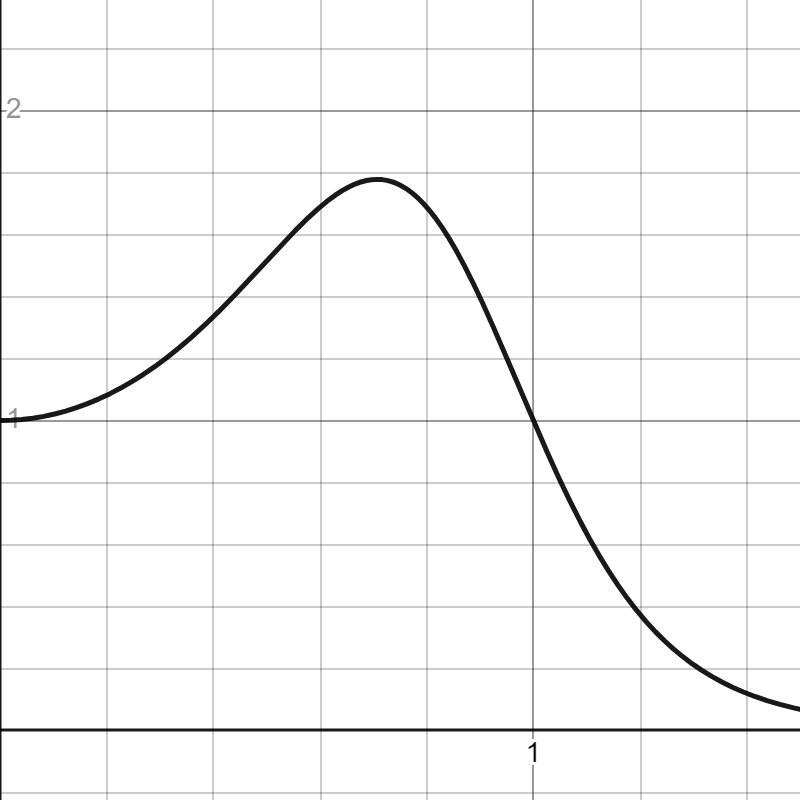
\includegraphics[width=0.4\textwidth]{hypothesis.png}
    \caption{Amplitude of forced pendulum as a function of angular frequency of the driver pendulum graph using Desmos to present a hypothesis of the function's curve shape}
    \label{fig:hypothesis}
\end{figure}

\section{Materials}

\begin{paracol}{2}
    \begin{itemize}
        \item (3) Retort Stands
        \item (2) C-clamps
        \item (4) Clamps
        \item \(\SI{11}{cm} \pm \SI{0.5}{cm}\) ruler
        \item \(\SI{15}{cm} \pm \SI{0.5}{cm}\) ruler
        \item (2) Meter Sticks
        \item (1) \SI{200}{g} weight
    \end{itemize}
    \switchcolumn
    \begin{itemize}
        \item (1) \SI{50}{g} weight
        \item Tape
        \item String
        \item Paper
        \item Scissors
        \item Highlighter
        \item Phone Camera
    \end{itemize}
\end{paracol}

\section{Variables}

\subsection{Independent Variable}
The independent variable is the angular frequency of the driver pendulum
/\unit{rad.s^{-1}}. In this lab, the independent variable will be changed
by shortening the length of the string. This change will be measured by
PASCO Capstone's distance measurement tool.

\subsection{Dependent Variable}
The dependent variable is the amplitude of the forced pendulum /\unit{rad}.
The dependent variable will be measured using PASCO Capstone's
object tracking tool.

\subsection{Controlled Variables}

The first controlled variable will be the starting amplitude of the
driver pendulum. This variable will be controlled by setting up a
meter stick with its foot pivoted on a retort stand at a
consistent position while leaning on the meter stick
sitting on top of the clamps between the two primary retort
stands, where each trial involved pushing the driver pendulum up to the
angle of that leaning meter stick. This variable must be controlled in
order to ensure that any changes in the amplitude of the forced
pendulum between trials isn't a result of varying
initial amplitude of the
driver pendulum and therefore inconsistent total energy in the system.
This controlled variable is also seen in Equation \ref*{eq:unlinearized}
from \(C = \frac{A_e}{ml}\), where \(A_e\) is the
amplitude of the external periodic force.

The second controlled variable will be the tension in the
master string that both pendulums are suspended from. This variable
will be controlled by using the same string of a consistent length
and maintaining the positions of the primary retort
stands with C-clamps. This variable must be controlled to
ensure that the degree of energy exchange between the
two pendulums is consistent between trials. Additionally,
overly loose strings will cause the degree of oscillation
in the master string to drastically effect the data.

The third controlled variable is the length of the
forced pendulum. This variable will be controlled by not
exchanging the string of the forced pendulum between trials.
This variable must be controlled to ensure that the
angular frequency of the forced pendulum seen
in Equation \ref*{eq:unlinearized} as \(\omega\)
remains consistent. It also ensures that \(C\)
remains consistent as \(C = \frac{A_e}{ml}\),
where \(l\) is the length of the forced pendulum.

The fourth controlled variable is the mass of
the forced pendulum. This variable will be controlled by
avoiding the exchange of weights of different
masses for the forced pendulum between trials.
This variable must be controlled to
ensure that the parameters of \(C = \frac{A_e}{ml}\)
and \(\lambda = \frac{\gamma}{m}\) remain consistent.

\section{Safety, Ethical, and Environmental Considerations}

There were no ethical or environmental issues in
this lab. A safety consideration is to avoid
excessive tightening of the C-clamp such that
the retort stand's base buckles. Another
safety consideration is to carry long objects
(e.g. meter sticks, retort stands) such that
they will not impact delicate objects
or others in the lab.

\section{Experimental Protocol}

A string was cut using scissors to a length
that is slightly longer than a meter stick.
A good portions of the ends were folded and twisted
to create a loop at the ends. Two clamps were positioned
near the top of two retort stands where the loops were
wrapped around the clamps' screws.


The retort stands were separated
as much as possible such that the
master string would have as much
tension as possible. The retort stands
were then secured using the C-clamps.
With
the bases of the two stands oriented with
the rods as far away as possible from each other,
the edges of the bases were observed to be \SI{53}{cm}
apart.

The \SI{200}{g} weight was dedicated to be the
driver pendulum and the \SI{50}{g} weight was dedicated
to be the forced pendulum. The motivation of this configuration
was that if the driver pendulum had significantly more
mass to it, then it would be resistant to complete
energy transfers to the forced pendulum.
A slip of paper was coloured with pink highlighter
and was wrapped around the \SI{50}{g} weight. The
purpose of doing this was so PASCO Capstone can
easily track the forced pendulum.

A string of some arbitrary length was cut and
was attached to the forced pendulum and suspended
from the master using loops. A triangular ruler
was then taped onto the third retort stand,
in which the height of the triangular ruler was
\SI{11}{cm}. Using 2 clamps to secure the phone onto one
of the primary retort stands, the forced pendulum
and the third retort stand were aligned in the
same plane, and a picture was taken using the phone.
The motivation of this was to analyse
that image using PASCO to determine
a more accurate length that
considers the centre of mass of the weight.

A longer string length was then attached
to the \SI{200}{g} weight for the driving
pendulum and suspended on the master string.
The forced pendulum was shifted along the
master string towards the side of the retort
stand with the phone, and the driver pendulum
was suspended on the side of the other
retort stand. The third retort stand
was aligned along the plane of the
driver pendulum. A meter stick was placed
on top of the two clamps securing the master
string and another meter stick was
set to lean against the first meter stick
with its foot sitting against the base
of the third retort stand. The motivation
of this set up was to maintain a consistent
initial amplitude of the driver
pendulum, therefore a \SI{15}{cm}
ruler sat between the two
retort stands to ensure that the distance between
the two bases are consistent.

Each trial involved setting the phone
to record the motion of the forced
pendulum after releasing the driver
pendulum. Changing the driver pendulum's
length involved increasing the size of the loop
such that the overall length is reduced.
If the length reaches the point where
there is too much excess string, then
some string was cut off to allow this process
to continue.

\begin{figure}[H]
    \centering
    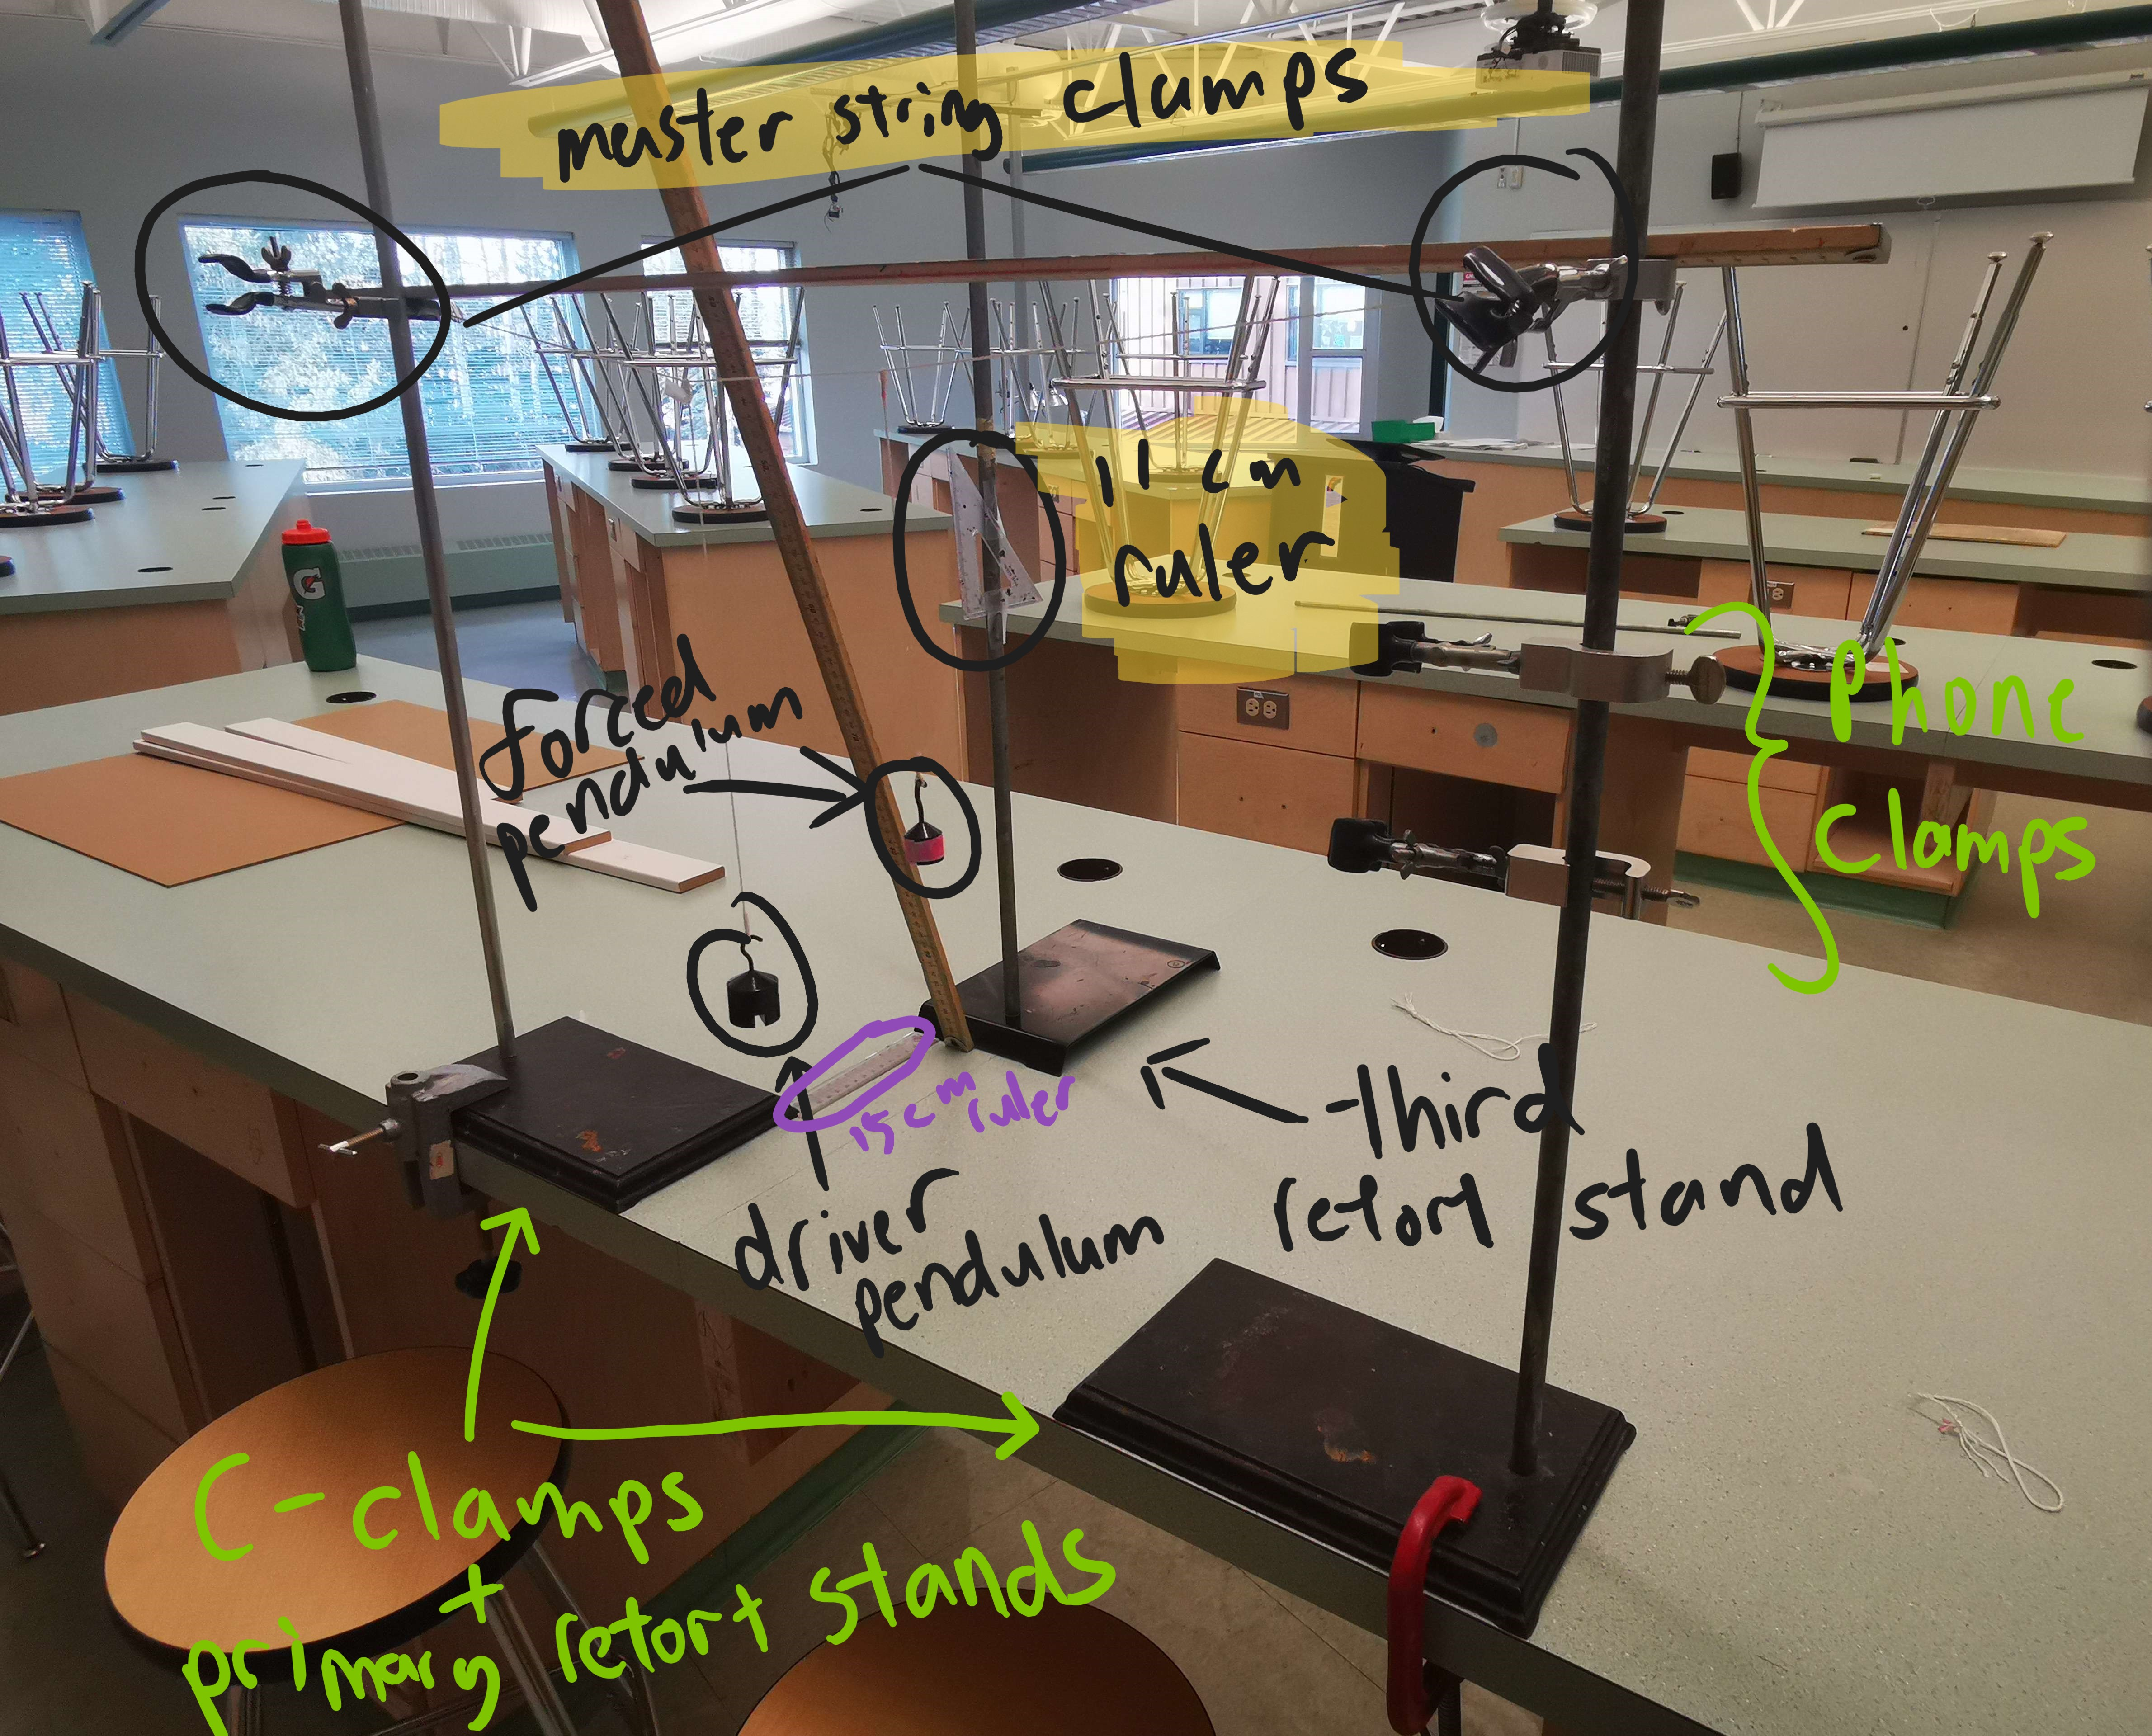
\includegraphics[width=0.7\textwidth]{entireSetup.jpg}
    \caption{Lab experiment apparatus setup}
    \label{fig:entireSetup}
\end{figure}

%TODO: data processing process

\section{Raw Data}

\subsection{Qualitative Observations}

\begin{itemize}
    \item As the angular frequency of the driver pendulum approached the resonant angular frequency of the forced pendulum, the driver pendulum experiences progressively more complete energy transfers. This was observed as temporary absence of potential and kinetic energy in the driver pendulum when the forced pendulum experiences oscillations of maximum amplitude.
    \item As the angular frequency of the driver pendulum approached the resonant angular frequency of the forced pendulum, the period that the forced pendulum transitions from no energy to maximum energy back to no energy increased.
    \item Despite the method of controlling the tension of the master string by avoiding exchange between different master strings, the string was observed to lose tension overtime.
    \item When the length of the driver pendulum was \SI{0.156}{m}, the master string failed and collapsed.
\end{itemize}

\subsection{Quantitative Data}

Table \ref*{tab:rawData} presents the raw data collected from the
experiment that are necessary to determine the angular frequency
of the driver pendulum and the maximum amplitude of the forced
pendulum for each trial.

\begin{table}[H]
    \centering
    \caption{Average, maximum, and minimum horizontal oscillation position and maximum and minimum vertical oscillation position as functions of the length of driver pendulum}
    \label{tab:rawData}
    \begin{tblr}{
        width = \linewidth,
        colspec = {Q[202]Q[165]Q[144]Q[144]Q[144]Q[138]},
        cells = {c},
        hlines,
        vlines,
        }
        {Length of
        driver                                                                                                       \\pendulum /$\unit{m}$} & {Average of horizontal\\oscillation position /$\unit{mm}$} & {Maximum of horizontal\\oscillation position /$\unit{mm}$} & {Minimum of horizontal\\oscillation position /$\unit{mm}$} & {Maximum of vertical\\oscillation position /$\unit{mm}$} & Minimum of vertical oscillation position /$\unit{mm}$\\
        $0.374 \pm 0.007$ & $-2.24 \pm 0.04$ & $39.5 \pm 0.7$ & $-45.0 \pm 0.8$ & $2.50 \pm 0.05$ & $-7.9 \pm 0.1$   \\
        $0.353 \pm 0.006$ & $-15.1 \pm 0.3$  & $39.7 \pm 0.7$ & $-67 \pm 1$     & $4.62 \pm 0.08$ & $-4.32 \pm 0.08$ \\
        $0.320 \pm 0.006$ & $-10.2 \pm 0.2$  & $62 \pm 1$     & $-86 \pm 2$     & $2.50 \pm 0.05$ & $-7.9 \pm 0.1$   \\
        $0.297 \pm 0.005$ & $-13.2 \pm 0.2$  & $70 \pm 1$     & $-95 \pm 2$     & $7.2 \pm 0.1$   & $-7.7 \pm 0.1$   \\
        $0.269 \pm 0.005$ & $-14.1 \pm 0.3$  & $104 \pm 2$    & $-129 \pm 2$    & $17.6 \pm 0.3$  & $-6.6 \pm 0.1$   \\
        $0.250 \pm 0.005$ & $-12.9 \pm 0.2$  & $134 \pm 2$    & $-157 \pm 3$    & $26.1 \pm 0.5$  & $-9.1 \pm 0.2$   \\
        $0.240 \pm 0.004$ & $-13.7 \pm 0.2$  & $177 \pm 3$    & $-204 \pm 4$    & $51.6 \pm 0.9$  & $-6.6 \pm 0.1$   \\
        $0.229 \pm 0.004$ & $-13.8 \pm 0.3$  & $205 \pm 4$    & $-229 \pm 4$    & $75 \pm 1$      & $-9.3 \pm 0.2$   \\
        $0.203 \pm 0.004$ & $-13.1 \pm 0.2$  & $193 \pm 4$    & $-211 \pm 4$    & $63 \pm 1$      & $-9.1 \pm 0.2$   \\
        $0.168 \pm 0.003$ & $-15.0 \pm 0.3$  & $114 \pm 2$    & $-138 \pm 3$    & $25.1 \pm 0.5$  & $-9.6 \pm 0.2$   \\
        $0.156 \pm 0.003$ & $-18.0 \pm 0.3$  & $91 \pm 2$     & $-129 \pm 2$    & $21.9 \pm 0.4$  & $-7.3 \pm 0.1$   \\
        $0.153 \pm 0.003$ & $-18.6 \pm 0.3$  & $88 \pm 2$     & $-122 \pm 2$    & $20.6 \pm 0.4$  & $-7.7 \pm 0.1$   \\
        $0.130 \pm 0.002$ & $-10.8 \pm 0.2$  & $69 \pm 1$     & $-90 \pm 2$     & $13.3 \pm 0.2$  & $-6.6 \pm 0.1$   \\
        $0.212 \pm 0.004$ & $8.0 \pm 0.1$    & $197 \pm 4$    & $-233 \pm 4$    & $74 \pm 1$      & $-7.7 \pm 0.1$   \\
        $0.115 \pm 0.002$ & $-17.9 \pm 0.3$  & $57 \pm 1$     & $-88 \pm 2$     & $10.7 \pm 0.2$  & $-7.6 \pm 0.1$
    \end{tblr}
\end{table}

The uncertainty for each value was dependent on the uncertainty
of the ruler used for PASCO Capstone to use as a reference
length. Because the calibration of the ruler
relied on orienting points based off of pixels,
the confidence and uncertainty of one
position along the ruler is
the increment of length for each tick
on the ruler (\(\pm \SI{1}{mm}\)).
However, because the overall
calibration of the ruler's length
involves two points, then the
final uncertainty for the \SI{11.0}{cm}
ruler is \(\pm \SI{0.2}{cm}\).

Because this uncertainty
is relative to the \SI{11.0}{cm}
ruler, then the uncertainties
for the distance measurements according to PASCO Capstone
will be the percent uncertainty of the ruler.
A sample calculation is shown below for the
length of the driver pendulum of the first trial.

\begin{align*}
    \text{Let } l_e & = \text{the length of the external driver pendulum } /\unit{m}
    \\
    l_r             & = \text{the length of the reference ruler } /\unit{cm}
    \\
    \Delta l_e      & = l_e \left( \frac{\Delta l_r}{l_r} \right)
    \\
                    & = (\SI{0.374}{m}) \left( \frac{\SI{0.2}{cm}}{\SI{11.0}{cm}} \right)
    \\
                    & = \SI{0.007}{m}
\end{align*}

\section{Processed Data}

The lengths of the driver pendulums will be used to determine
the angular frequency of the driver pendulum for each trial.
A sample calculation is shown below for the length of the
driver pendulum of the first trial.

\begin{paracol}{2}
    \begin{align*}
        \Omega & = \sqrt{\frac{g}{l_e}}
        \\
               & = \sqrt{\frac{\SI{9.81}{m.s^{-2}}}{\SI{0.374}{m} \pm \SI{0.007}{m}}}
        \\
               & = \SI{5.12}{rad.s^{-1}} \pm \SI{0.05}{rad.s^{-1}}
    \end{align*}
    \switchcolumn
    From \cite{gonzalesMeasurementUncertaintySquares2022}
    \begin{align*}
        \Delta \Omega & = \Omega \left( \frac{1}{2} \cdot \frac{\Delta l_e}{l_e} \right)
        \\
                      & = (\SI{5.12}{rad.s^{-1}})\left( \frac{1}{2} \cdot \frac{\SI{0.007}{m}}{\SI{0.374}{m}} \right)
        \\
                      & = \SI{0.05}{rad.s^{-1}}
    \end{align*}
\end{paracol}

Next, based on the maximum, minimum, and average
positions of the pendulum along the horizontal and
vertical axis can be used to determine
the pendulum's maximum horizontal and vertical
displacement from equilibrium.
For the horizontal axis, its maximum
distance from equilibrium is the greater
value between \(|X_{max} - X_{average}\)
and \(|X_{min} - X_{average}|\).
For the vertical axis, its
maximum distance from equilibrium is
\(|Y_{max} - Y_{min}|\).

\begin{figure}[H]
    \centering
    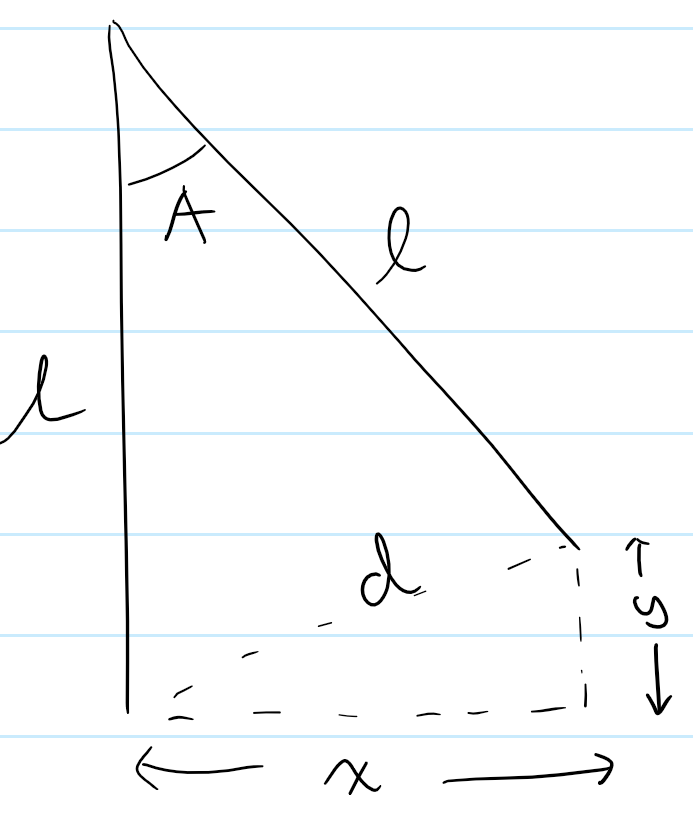
\includegraphics[width=0.4\textwidth]{determineAmplitude.png}
    \caption{Forced pendulum at its maximum amplitude labelled with relevant variables to determine the value of the maximum amplitude}
    \label{fig:determineAmplitude}
\end{figure}

The amplitude of the forced pendulum /\unit{rad} can be determined
by taking the maximum horizontal oscillation amplitude
and the maximum vertical oscillation amplitude
and using cosine law to determine the angle
that the forced pendulum has rotated about its
pivot. The calculation for this for the first
trial is shown below with reference to Figure \ref*{fig:determineAmplitude}.

\begin{align*}
    \text{Let } l & = \text{the length of the forced pendulum }
    \\
    d^2           & = 2l^2 - 2l^2\cos A,\quad d^2 = x^2 + y^2
    \\
    A             & = \arccos \left( 1 - \frac{x^2 + y^2}{2l^2} \right)
    \\
                  & = \arccos \left( 1 - \frac{( \SI{4.27}{cm} \pm \SI{0.09}{cm} )^2 + (\SI{1.04}{cm} \pm \SI{0.02}{cm})^2}{2(\SI{26.1}{cm} \pm \SI{0.5}{cm})^2 } \right)
    \\
                  & = \SI{0.168}{rad}
    \\
                  & \text{Using Equation \ref*{eq:partialUnc} to propagate the uncertainty}
    \\
    A             & = \SI{0.168}{rad} \pm \SI{0.006}{rad}
\end{align*}

\begin{align}
    \text{From}                     & \text{ \cite{UncertaintiesErrorPropagation}} \nonumber
    \\
    \Delta f(a_1, a_2, a_3, \cdots) & = \sum \left| \pdv{f}{a_n} \right| \Delta a_n \label{eq:partialUnc}
    \\
    \text{Where } f                 & = \text{the multivariable function whose uncertainty is to be found} \nonumber
    \\
    a_n                             & = \text{the nth variable in f} \nonumber
\end{align}

Table \ref*{tab:processedData} presents the processed data
that will provide the necessary values to graph the
relationship between the forced pendulum's maximum
amplitude and the angular frequency of the driver
pendulum.

\begin{table}[H]
    \centering
    \caption{Maximum horizontal and vertical displacement from equilibrium of forced pendulum and maximum amplitude of forced pendulum as a function of the angular frequency of the driver pendulum }
    \label{tab:processedData}
    \begin{tblr}{
        width = \linewidth,
        colspec = {Q[200]Q[250]Q[250]Q[242]},
        cells = {c},
        hlines,
        vlines,
        }
        {Angular
        frequency of                                                            \\driver pendulum /$\unit{rad.s^{-1}}$} & {Forced pendulum's maximum horizontal displacement\\from equilibrium /$\unit{cm}$} & {Forced pendulum's maximum vertical displacement\\from equilibrium /$\unit{cm}$} & Forced pendulum's maximum amplitude /$\unit{rad}$ \\
        $5.12 \pm 0.05$ & $4.27 \pm 0.09$ & $1.04 \pm 0.02$ & $0.168 \pm 0.006$ \\
        $5.27 \pm 0.05$ & $5.5 \pm 0.1$   & $0.89 \pm 0.02$ & $0.213 \pm 0.008$ \\
        $5.54 \pm 0.05$ & $7.6 \pm 0.2$   & $1.04 \pm 0.02$ & $0.30 \pm 0.01$   \\
        $5.75 \pm 0.05$ & $8.3 \pm 0.2$   & $1.49 \pm 0.03$ & $0.33 \pm 0.01$   \\
        $6.04 \pm 0.05$ & $11.9 \pm 0.2$  & $2.42 \pm 0.04$ & $0.47 \pm 0.02$   \\
        $6.26 \pm 0.06$ & $14.6 \pm 0.3$  & $3.51 \pm 0.06$ & $0.58 \pm 0.02$   \\
        $6.39 \pm 0.06$ & $19.1 \pm 0.3$  & $5.8 \pm 0.1$   & $0.78 \pm 0.03$   \\
        $6.55 \pm 0.06$ & $21.9 \pm 0.4$  & $8.5 \pm 0.2$   & $0.93 \pm 0.04$   \\
        $6.96 \pm 0.06$ & $20.6 \pm 0.4$  & $7.2 \pm 0.1$   & $0.86 \pm 0.03$   \\
        $7.64 \pm 0.07$ & $12.9 \pm 0.2$  & $3.48 \pm 0.06$ & $0.52 \pm 0.02$   \\
        $7.93 \pm 0.07$ & $11.1 \pm 0.3$  & $2.92 \pm 0.05$ & $0.44 \pm 0.02$   \\
        $8.00 \pm 0.07$ & $10.7 \pm 0.2$  & $2.83 \pm 0.05$ & $0.43 \pm 0.02$   \\
        $8.69 \pm 0.08$ & $8.0 \pm 0.1$   & $1.99 \pm 0.04$ & $0.32 \pm 0.01$   \\
        $6.80 \pm 0.06$ & $24.1 \pm 0.4$  & $8.1 \pm 0.1$   & $1.02 \pm 0.04$   \\
        $9.24 \pm 0.08$ & $7.5 \pm 0.1$   & $1.83 \pm 0.03$ & $0.29 \pm 0.01$
    \end{tblr}
\end{table}

Table \ref*{tab:analysisData} presents the reciprocal of the forced
pendulum's maximum amplitude squared as a function of the
square of the angular frequency of the driver pendulum.
Note that Equation \ref*{eq:partialUnc} was used to
propagate the uncertainties of the values in the table.

\begin{table}[H]
    \centering
    \caption{Reciprocal of the forced pendulum's maximum amplitude squared as a function of the square of the angular frequency of the driver pendulum}
    \label{tab:analysisData}
    \begin{tblr}{
        width = \linewidth,
        colspec = {Q[490]Q[452]},
        cells = {c},
        hlines,
        vlines,
        }
        {Square of angular frequency of    \\driver pendulum /$\unit{rad^2.s^{-2}}$} & {Reciprocal of the forced pendulum's maximum amplitude squared /$\unit{rad^{-2}}$} \\
        $26.24 \pm 0.09$ & $35 \pm 3$      \\
        $27.8 \pm 0.1$   & $22 \pm 2$      \\
        $30.7 \pm 0.1$   & $11 \pm 1$      \\
        $33.0 \pm 0.1$   & $9.5 \pm 0.7$   \\
        $36.4 \pm 0.1$   & $4.6 \pm 0.3$   \\
        $39.2 \pm 0.1$   & $2.9 \pm 0.2$   \\
        $40.8 \pm 0.1$   & $1.6 \pm 0.1$   \\
        $42.9 \pm 0.1$   & $1.16 \pm 0.09$ \\
        $48.4 \pm 0.1$   & $1.3 \pm 0.1$   \\
        $58.4 \pm 0.1$   & $3.8 \pm 0.3$   \\
        $62.9 \pm 0.1$   & $5.1 \pm 0.4$   \\
        $64.0 \pm 0.1$   & $5.5 \pm 0.4$   \\
        $75.6 \pm 0.2$   & $10.1 \pm 0.7$  \\
        $46.2 \pm 0.1$   & $0.97 \pm 0.08$ \\
        $85.3 \pm 0.2$   & $11.5 \pm 0.8$
    \end{tblr}
\end{table}

\section{Analysis}

\begin{figure}[H]
    \centering
    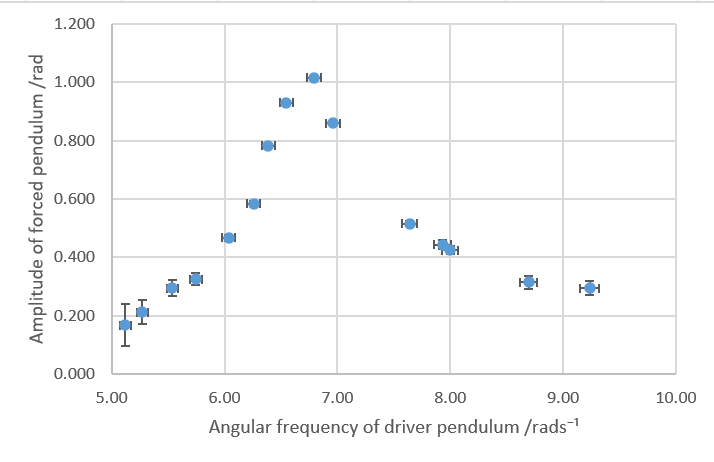
\includegraphics[width=0.6\textwidth]{defaultGraph.png}
    \caption{Amplitude of forced pendulum /\unit{rad} as a function of angular frequency of driver pendulum /\unit{rad.s^{-1}} to confirm the hypothesis to the research question}
    \label{fig:defaultGraph}
\end{figure}

As seen in Figure \ref*{fig:defaultGraph}, a portion of the hypothesis
has been proven, where there is a maximum in the graph
at when the driver pendulum's angular frequency resonates
with the forced pendulum's angular frequency.

Further analysis can be done given the graph in Figure \ref*{fig:fullGraphOfModified}.

\begin{figure}[H]
    \centering
    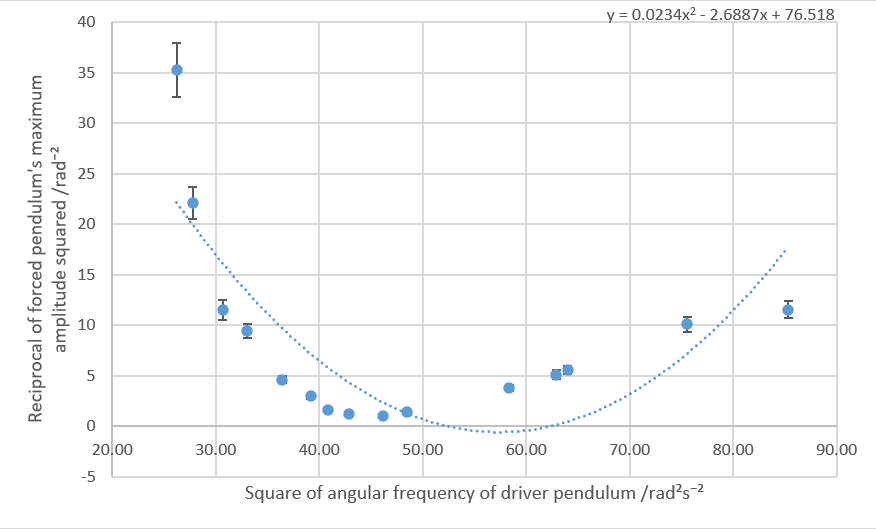
\includegraphics[width=0.7\textwidth]{fullGraphOfModified.png}
    \caption{Reciprocal of forced pendulum's maximum amplitude squared /\unit{rad^{-2}} as a function of square of angular frequency of driver pendulum /\unit{rad^2.s^{-2}} to indicate error in data}
    \label{fig:fullGraphOfModified}
\end{figure}

Evidently, this trend does not fit the parabolic model discussed
earlier. However, further inspection may suggest that
the first portion follows a trend resembling one
that is quadratic, with the final 5 data points
breaking the trend. By restricting the data points
to not include the final 5 values, a
graph is produced that better fits the parabolic model,
as seen in Figure \ref*{fig:restrictedGraph}.

\begin{figure}[H]
    \centering
    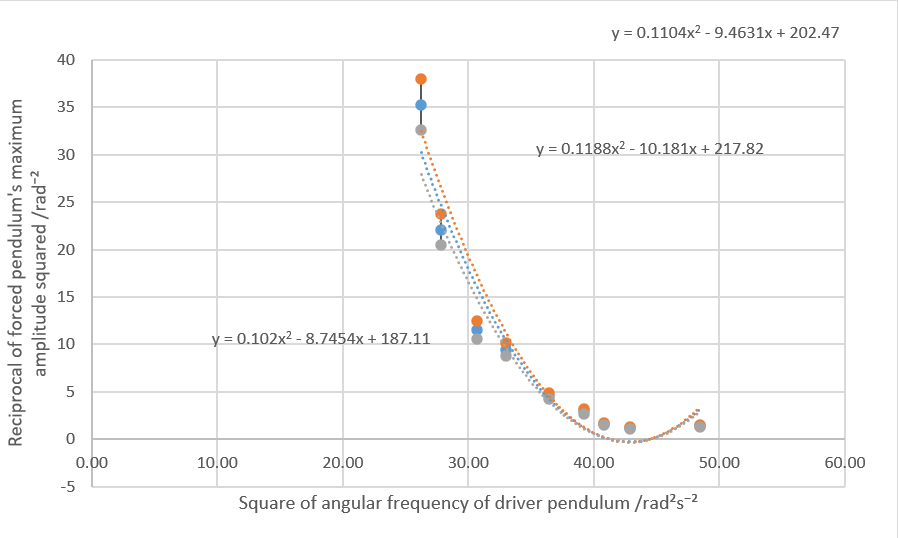
\includegraphics[width=0.7\textwidth]{restrictedGraph.png}
    \caption{Reciprocal of forced pendulum's maximum amplitude squared /\unit{rad^{-2}} as a function of square of angular frequency of driver pendulum /\unit{rad^2.s^{-2}} to focus on the portion of the data that best follows the parabolic model}
    \label{fig:restrictedGraph}
\end{figure}

The parameters of the best-fit parabola can be
used in conjunction with Equation \ref*{eq:unlinearized}
to quantify the data's accuracy. Specifically,
the parameters can be used to experimentally determine
the forced pendulum's angular frequency, which is
comparable to a theoretical value obtained by \(\omega = \sqrt{\frac{g}{l}}\).

The following parabolic relationship is formed from the
topmost trend and lowest trend maximized and minimized
respectively according to y-intercept which
is the most significant parameter to determining
the experimental angular frequency of the forced pendulum.

\begin{equation}
    \frac{1}{A^2} = ( \SI{0.110}{s^4} \pm \SI{0.008}{s^4} )\Omega^4 - ( \SI{9.5}{rad^2.s^{-2}} \pm \SI{0.7}{rad^2.s^{-2}} )\Omega^2 + ( \SI{2.0e2}{rad^4} \pm \SI{0.2e2}{rad^4} )
\end{equation}

The experimental and theoretical angular frequencies of the forced pendulum can be
determined as shown below.

\begin{align*}
    \frac{1}{C^2}                                  & = \SI{0.110}{s^4} \pm \SI{0.008}{s^4},\quad \frac{\omega^4}{C^2} = \SI{2.0e2}{rad^4} \pm \SI{0.2e2}{rad^4}
    \\
    \omega^4 \left( \frac{1}{C^2} \right)          & = \SI{2.0e2}{rad^4} \pm \SI{0.2e2}{rad^4}
    \\
    \omega^4 (\SI{0.110}{s^4} \pm \SI{0.008}{s^4}) & = \SI{2.0e2}{rad^4} \pm \SI{0.2e2}{rad^4}
    \\
    \omega                                         & = \SI{6.5}{rad.s^{-1}} \pm \SI{0.3}{rad.s^{-1}}
    \\
    \\
    \omega_{theoretical}                           & = \sqrt{\frac{g}{l}}
    \\
                                                   & = \sqrt{\frac{\SI{9.81}{m.s^{-2}}}{\SI{0.261}{m} \pm \SI{0.005}{m}}}
    \\
                                                   & = \SI{6.13}{rad.s^{-1}} \pm \SI{0.06}{rad.s^{-1}}
\end{align*}

\section{Evaluation}

The experimental and theoretical values of the
angular frequency of the forced pendulum at a glance
look very close; however, the ranges defined by their
uncertainties barely intersect (\SI{6.2}{rad.s^{-1}} and \SI{6.19}{rad.s^{-1}}). This indicates that
the data collected in the experiment isn't the most accurate.
This was already evident in Figure \ref*{fig:defaultGraph} where
the final 5 data points break the quadratic trend.
While one may argue that the holistic trend
could be cubic, the theory only backs up the argument
that the relationship between \(\frac{1}{A^2}\) and \(\Omega^2\)
is quadratic. Despite this, further investigation
is required to confirm the portion of the hypothesis
predicting that this relationship is quadratic.

\subsection{Strengths}

Most experiments investigating an external periodic
force applied to a simple harmonic motion system
are done by using a motor to provide the external
periodic force. However, this experiment does
not necessitate the need to design a motor, as
the external periodic force is provided by
the driver pendulum that can be easily
made by anyone.

\subsection{Sources of Error}

The first source of error was the progressive decrease
in master string's tension overtime. Because of the
exaggerated amplitude of the forced pendulum
due to the additional master string's oscillation,
then it is expected that data points surrounding
the median of the angular frequencies of the driver
pendulum will have an amplitude that is higher
than reality. This in turn causes the
data points in the center of Figure \ref*{fig:restrictedGraph}
to be lower than reality. Assuming that the first
data point in Figure \ref*{fig:restrictedGraph}
remains static, then if all the other data points
were adjusted to be increased, than the y-intercept
would be expected to decrease. This in turn would
cause the experimental value of \(\omega\) to decrease
and therefore increase the likelihood that
the experimental value matches the theoretical value.
The first improvement is to layer the master string
with multiple strands such that the master string
is less prone to losing its tension. Another
improvement is to use a different material
for the master string such as fishing line
that is less prone to stretch overtime.

The second source of error was the master string's failure
when the length of the driver pendulum was \SI{0.156}{m}.
This explains the break in the trend in Figure \ref*{fig:defaultGraph},
as this was the 5th last data point that started the
break in the trend. The break in the trend was specifically
the way in which the 5 last data points fell under
the expected curve given by the best-fit parabola
of the rest of the data points, and this makes
sense given this source of error as because a loosened
string that was reattached to the retort stands
would allow for more energy transfer between the
pendulums and exaggerated oscillations due to the
master's string's additional oscillation, then
\(A\) would become larger than expected,
which in turn causes \(\frac{1}{A^2}\)
to be lower than expected. An improvement
to solve this source of error is to layer
the master string with multiple strands such
that the master string has increased durability
to avoid failure.


%TODO: extension of effect of changing position of pendulums along master string.

\bibliographystyle{apacite}
\bibliography{IB_PHYSICS_IA.bib}

\end{document}